\documentclass[onecolumn,draftclsnofoot, 10pt, compsoc]{IEEEtran}

\usepackage{graphicx}
\usepackage[section]{placeins}
\usepackage{caption}

\usepackage{amssymb}                                         
\usepackage{amsmath}                                         
\usepackage{amsthm}                                

\usepackage{alltt}                                           
\usepackage{float}
\usepackage{color}
\usepackage{url}

\usepackage{balance}
\usepackage[TABBOTCAP, tight]{subfigure}
\usepackage{enumitem}
\usepackage{pstricks, pst-node}
\usepackage{url}
\usepackage{setspace}

\usepackage{etoolbox}
\AtBeginEnvironment{quote}{\singlespacing\vspace{-\topsep}\small}

%\input{pygments.tex}

\usepackage{geometry}
\geometry{left=0.75in,right=0.75in,top=0.75in,bottom=0.75in}
\parindent = 0.0 in
\parskip = 0.1 in


\def \ParSpace{\vspace{.75em}}
\def \Jeremy{			Jeremy Fischer}
\def \Class{		Parallel Programming}
\def \Assn{		Project 6: OpenCL Array Multiply, Multiply-Add, and Multiply-Reduce}
\def \School{	Oregon State University}
\def \Professor{		Matthew Meyn}

\newcommand{\cred}[1]{{\color{red}#1}}
\newcommand{\cblue}[1]{{\color{blue}#1}}

\newcommand{\NameSigPair}[1]{
		\par
		\makebox[2.75in][r]{#1} \hfil 	\makebox[3.25in]{\makebox[2.25in]{\hrulefill} \hfill			
		\makebox[.75in]{\hrulefill}}
		\par\vspace{-12pt} \textit{
			\tiny\noindent
			\makebox[2.75in]{} \hfil		
			\makebox[3.25in]{
				\makebox[2.25in][r]{Signature} \hfill	\makebox[.75in][r]{Date}
			}
		}
}










%%%%%%%%%%%%%%%%%%%%%%%%%%%%%%%%%%%%%%%
\begin{document}
\begin{titlepage}
    \pagenumbering{gobble}
    \begin{singlespace}
    	
\includegraphics[height=4cm]{coe.eps}
        \hfill  
        \par\vspace{.2in}
        \centering
        \scshape{
            \vspace{.5in}
            \textbf{\Large\Assn}\par
            \textbf{\large\Class}\par
            \large{
            	\today \\Spring Term
        	}
            \vfill
            {\large Prepared for}\par
            \huge \School\par
            \vspace{5pt}
            {\Large{\Professor}\par}
            {\large Prepared by }\par

            \vspace{5pt}
            {\Large
                {\Jeremy}\par
            }
            \vspace{20pt}
        }

    \end{singlespace}
\end{titlepage}
\newpage
\pagenumbering{arabic}

% 7. uncomment this (if applicable). Consider adding a page break.
%\listoffigures
%\listoftables
\clearpage




\section{Array Multiply and Array Multiply and Add}
	\subsection{What machine you ran this on?}
		I ran this on \textit{rabbit.engr.oregonstate.edu}.
	
	
	\subsection{Results Table}
		\subsubsection{Array Multiplication}
			\begin{figure}[H]
				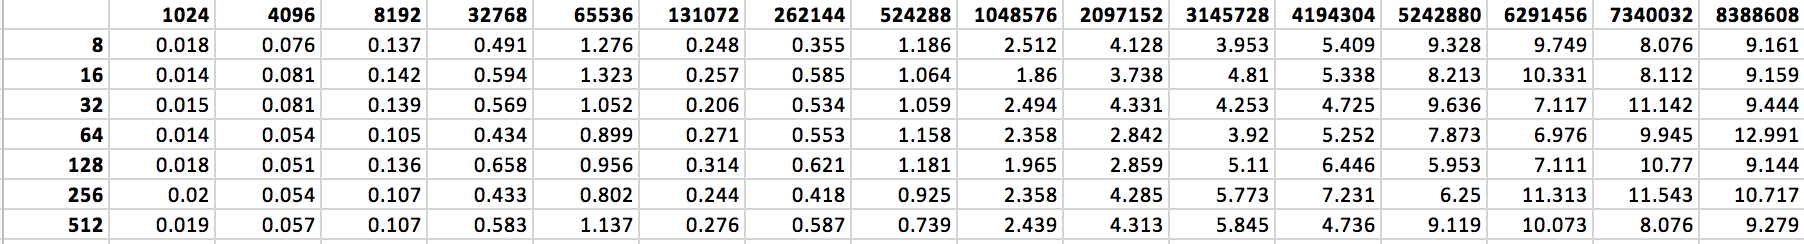
\includegraphics[width=18cm]{multTable}
				\centering
				\caption{A table of the \textit{Local Work Size} vs. \textit{Global Work Size} for the array multiplication program.
					The \textit{Local Work Size} is on the Y-axis in bold and the \textit{Global Work Size} is on the X-axis in bold}
			\end{figure}
	
		\subsubsection{Array Multiplication and Add}
			\begin{figure}[H]
				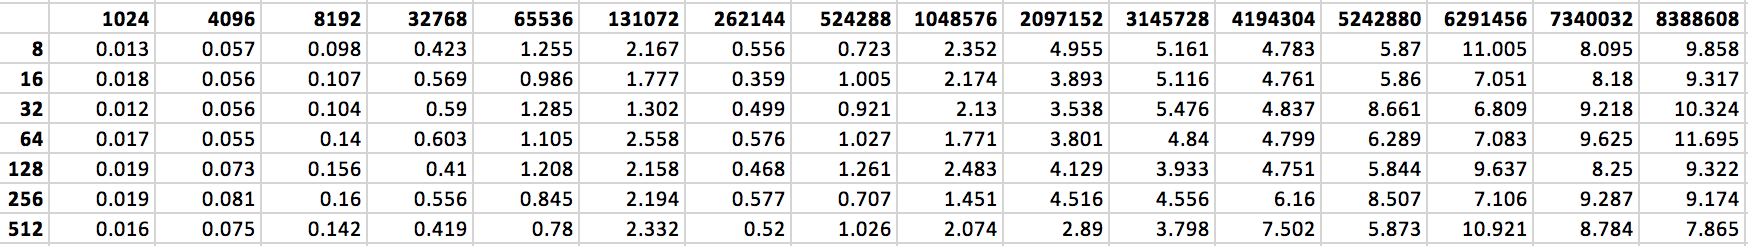
\includegraphics[width=18cm]{multAddTable}
				\centering
				\caption{A table of the \textit{Local Work Size} vs. \textit{Global Work Size} for the array multiplication and add program.
				 The \textit{Local Work Size} is on the Y-axis in bold and the \textit{Global Work Size} is on the X-axis in bold}
			\end{figure}
		
		
		
		
		
	\subsection{Results Graph}
		\subsubsection{Array Multiplication}
			\begin{figure}[H]
				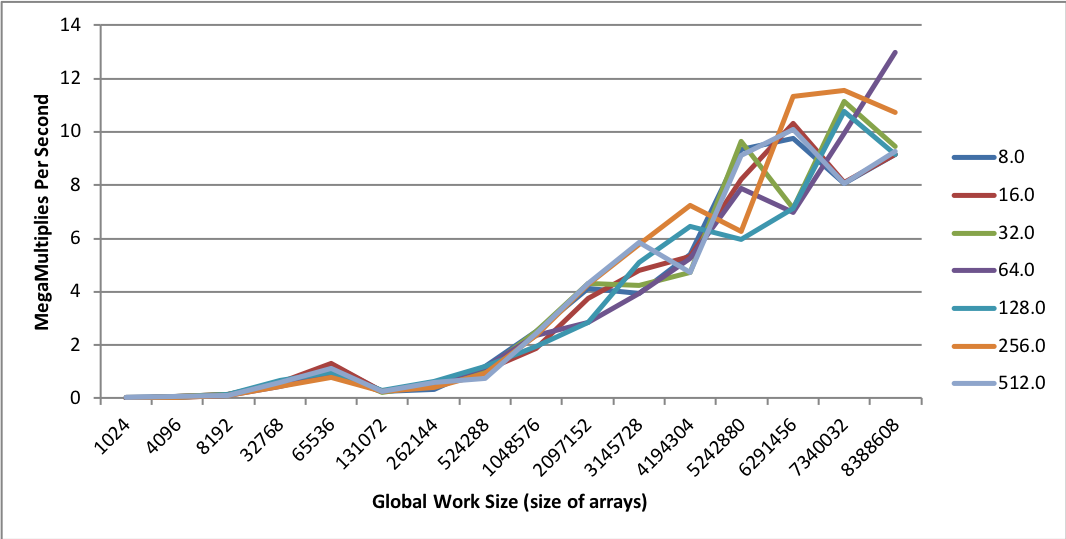
\includegraphics[width=16cm]{multMegasVsGlobal}
				\centering
				\caption{A graph of the \textit{Mega Multiplies Per Second} vs. \textit{Global Work Size} for the array multiplication program.}
			\end{figure}
				
			\begin{figure}[H]
				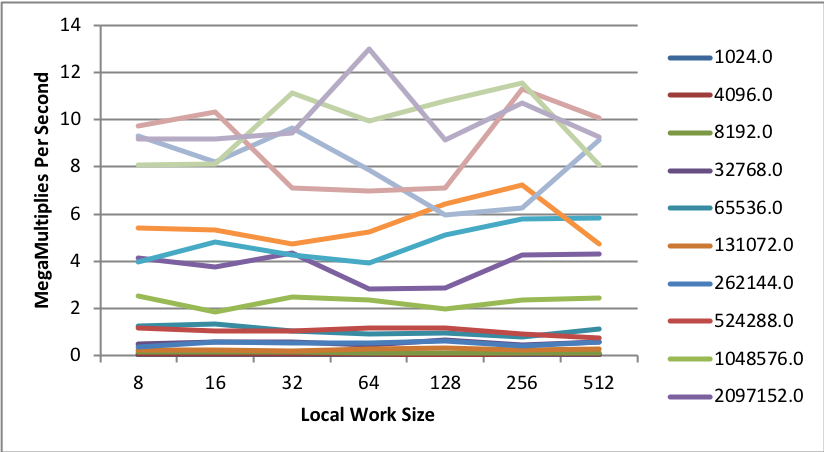
\includegraphics[width=16cm]{multMegasVsLocal}
				\centering
				\caption{A graph of the \textit{Mega Multiplies Per Second} vs. \textit{Local Work Size} for the array multiplication program.}
			\end{figure}
				
				
		\subsubsection{Array Multiplication and Add}
			\begin{figure}[H]
				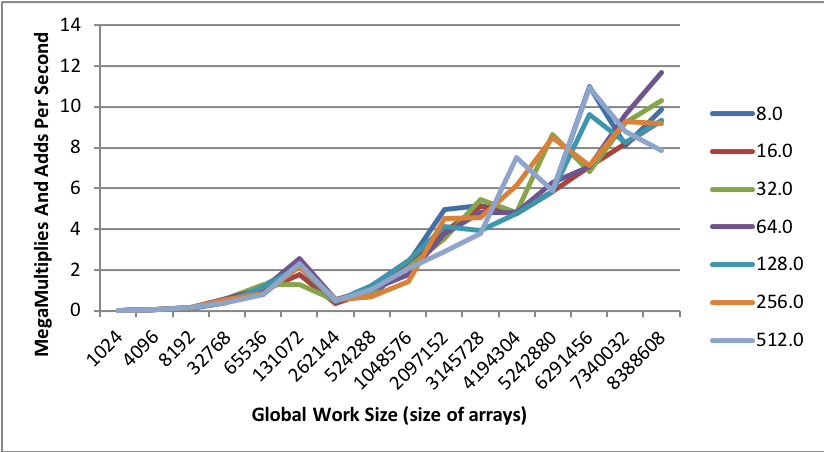
\includegraphics[width=16cm]{multAddMegasVsGlobal}
				\centering
				\caption{A graph of the \textit{Mega Multiplies And Adds Per Second} vs. \textit{Global Work Size} for the array multiplication and add program.}
			\end{figure}
			
			\begin{figure}[H]
				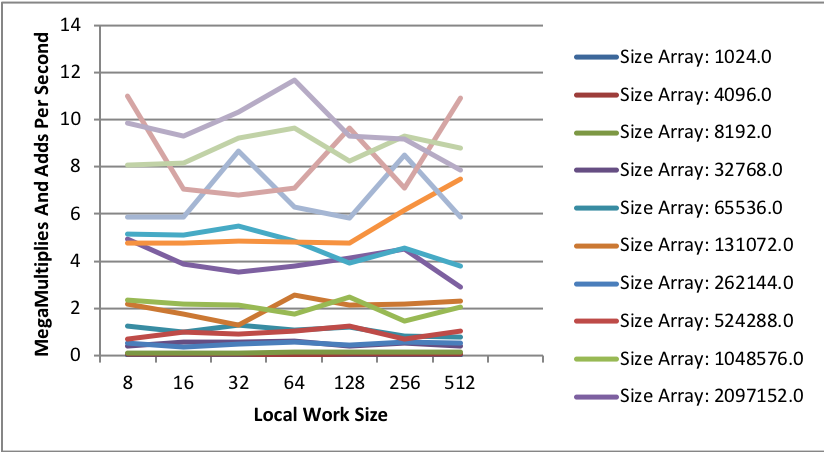
\includegraphics[width=16cm]{multAddMegasVsLocal}
				\centering
				\caption{A graph of the \textit{Mega Multiplies And Adds Per Second} vs. \textit{Local Work Size} for the array multiplication and add program.}
			\end{figure}

			
	









	\subsection{What patterns are you seeing in the performance curves?}

	
	
	
	
	
	
	
	
	\subsection{Why do you think the patterns look this way?}










	\subsection{What is the performance difference between doing a Multiply and doing a Multiply-Add?}
	
	





	
	
	
	\subsection{What does that mean for the proper use of GPU parallel computing?}









\section{Array Multiply With Reduction}
	\subsection{Results Table}
		\begin{figure}[H]
			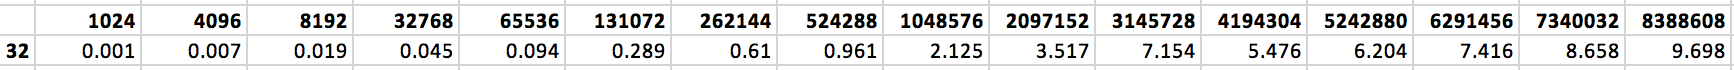
\includegraphics[width=18cm]{redTable}
			\centering
			\caption{A table of the \textit{Local Work Size} vs. \textit{Global Work Size} for the array multiplication with reduction program.
				The \textit{Local Work Size} is on the Y-axis in bold and the \textit{Global Work Size} is on the X-axis in bold}
		\end{figure}
	
	
	
	
	
	\subsection{Results Graph}
		\begin{figure}[H]
			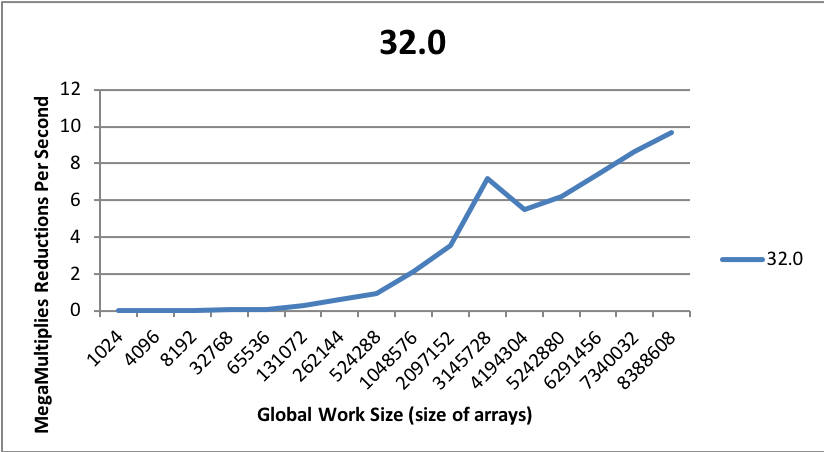
\includegraphics[width=16cm]{multRedMegasVsGlobal}
			\centering
			\caption{A graph of the \textit{Mega Multiplies With Reductions Per Second} vs. \textit{Global Work Size} for the array multiplication with reductions program.}
		\end{figure}




	
	
	
	\subsection{What pattern are you seeing in this performance curve?}
	
	
	
	
	
	
	
	
	
	\subsection{Why do you think the pattern looks this way?}
	
	
	
	
	
	
	
	
	
	\subsection{What does that mean for the proper use of GPU parallel computing?}
	





\end{document}